\chapter{Diagramas de flujo y secuencias de funcionamiento}
\label{anexo:diagramas_flujo_funcionamiento}

Este anexo resume los principales flujos de funcionamiento de TierraViva. Su finalidad es mostrar cómo se comporta el sistema durante una ejecución normal y ante situaciones de seguridad, sin repetir el detalle de instalación, estructura de ThingSpeak o referencia de la API, que se documentan en anexos específicos.

\section{Flujo general del sistema}

La Figura~\ref{fig:flujo_general_tierraviva} muestra el recorrido completo de la información desde la estación remota hasta el usuario.

\begin{figure}[H]
    \centering
    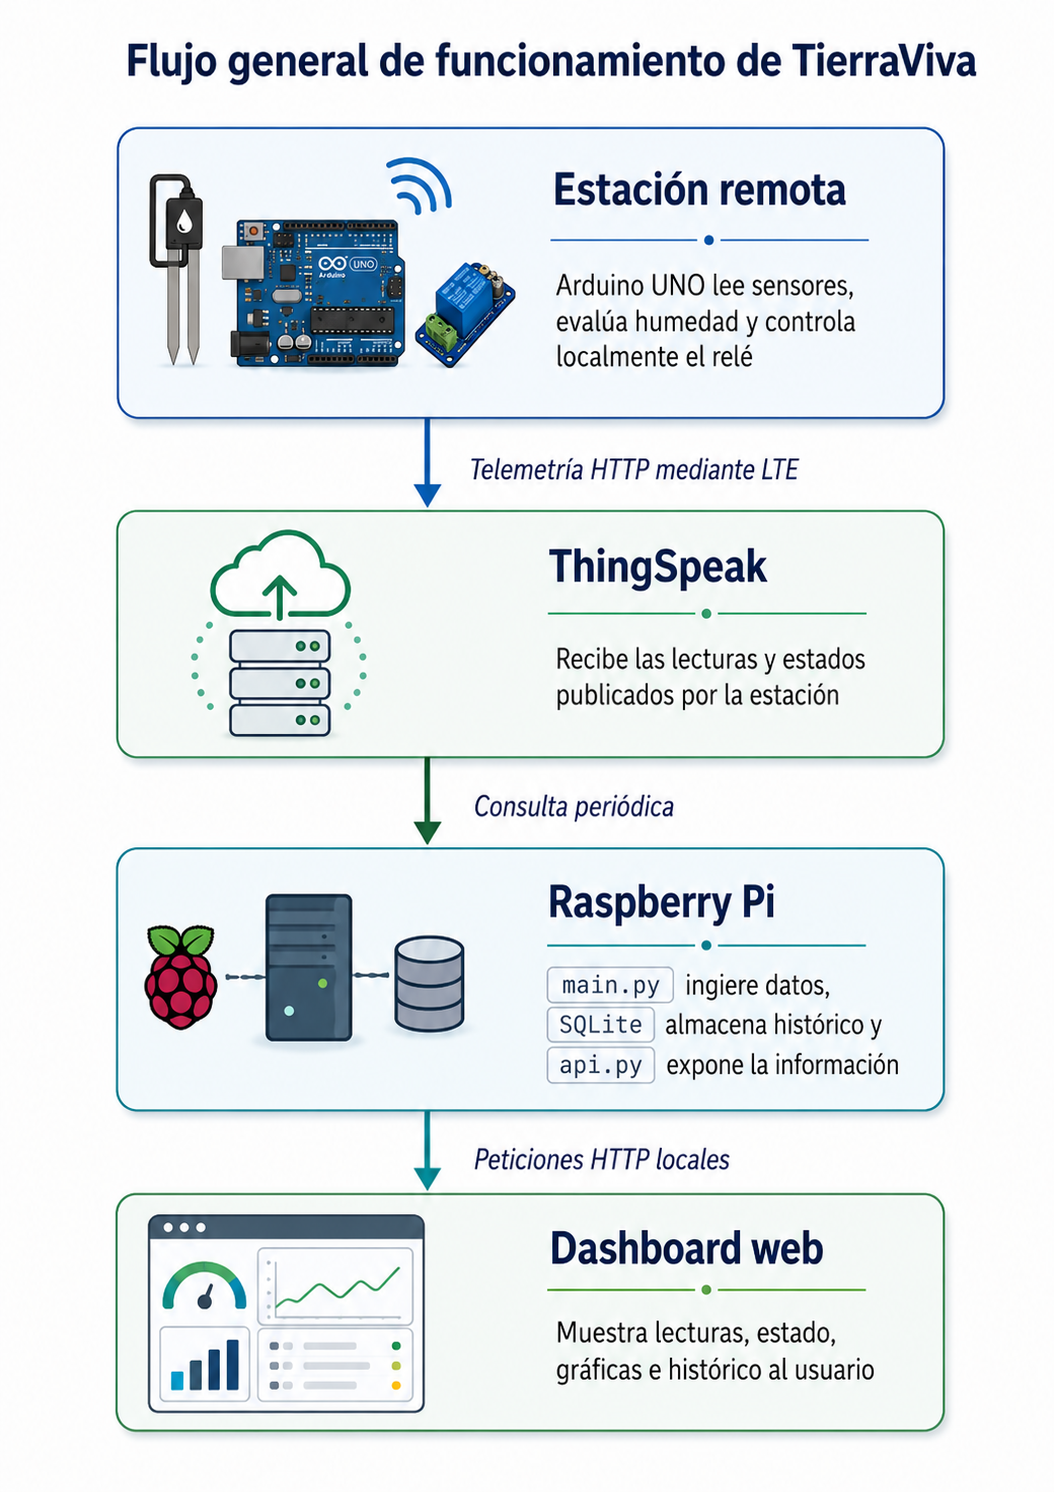
\includegraphics[width=0.5\textwidth]{figs_png/flujo_general_tierraviva.png}
    \caption{Flujo general de funcionamiento de TierraViva.}
    \label{fig:flujo_general_tierraviva}
\end{figure}

La estación concentra la medición, la decisión local y la actuación segura. ThingSpeak actúa como capa intermedia de telemetría, mientras que la Raspberry Pi se encarga de supervisar, almacenar y mostrar los datos.

\section{Ciclo de funcionamiento de la estación}

La Figura~\ref{fig:ciclo_estacion_tierraviva} resume el ciclo ejecutado por la estación remota.

\begin{figure}[H]
    \centering
    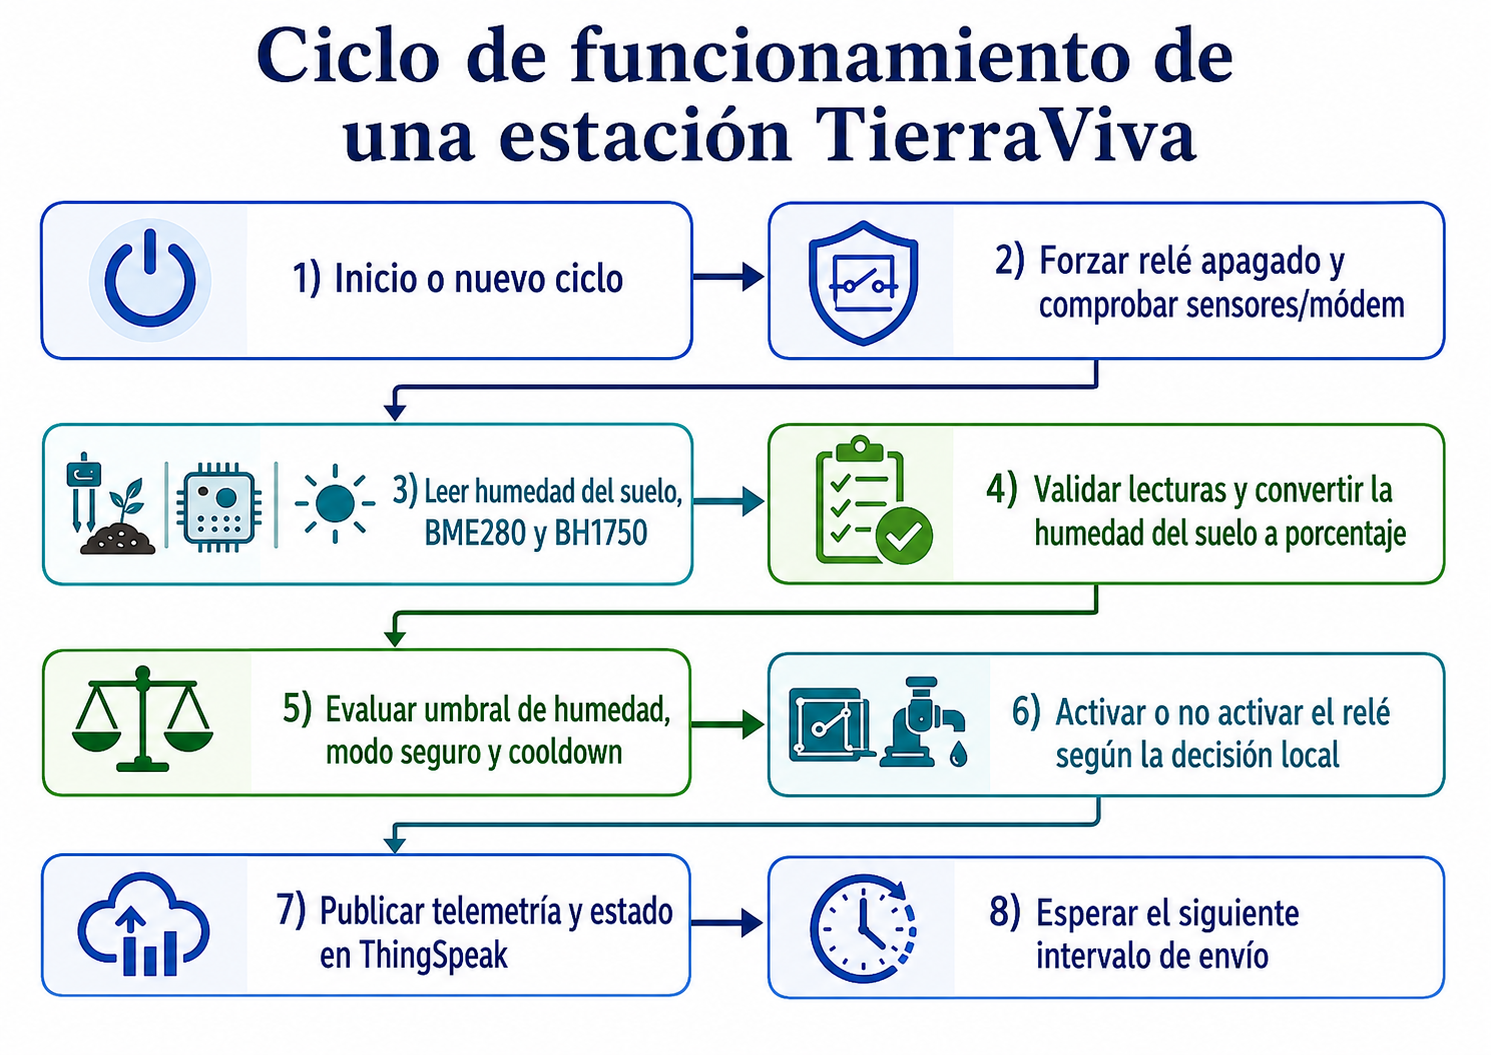
\includegraphics[width=\textwidth]{figs_png/ciclo_estacion_tierraviva.png}
        \caption{Ciclo de funcionamiento de una estación TierraViva.}
    \label{fig:ciclo_estacion_tierraviva}
\end{figure}

El relé se fuerza a estado apagado durante el arranque y la actuación se limita temporalmente mediante \textit{firmware}. Esta decisión reduce el riesgo de activaciones no deseadas.

\section{Decisión local de riego}

La Figura~\ref{fig:decision_local_riego_resumida} muestra la lógica principal de decisión de riego ejecutada en Arduino.

\begin{figure}[H]
    \centering
    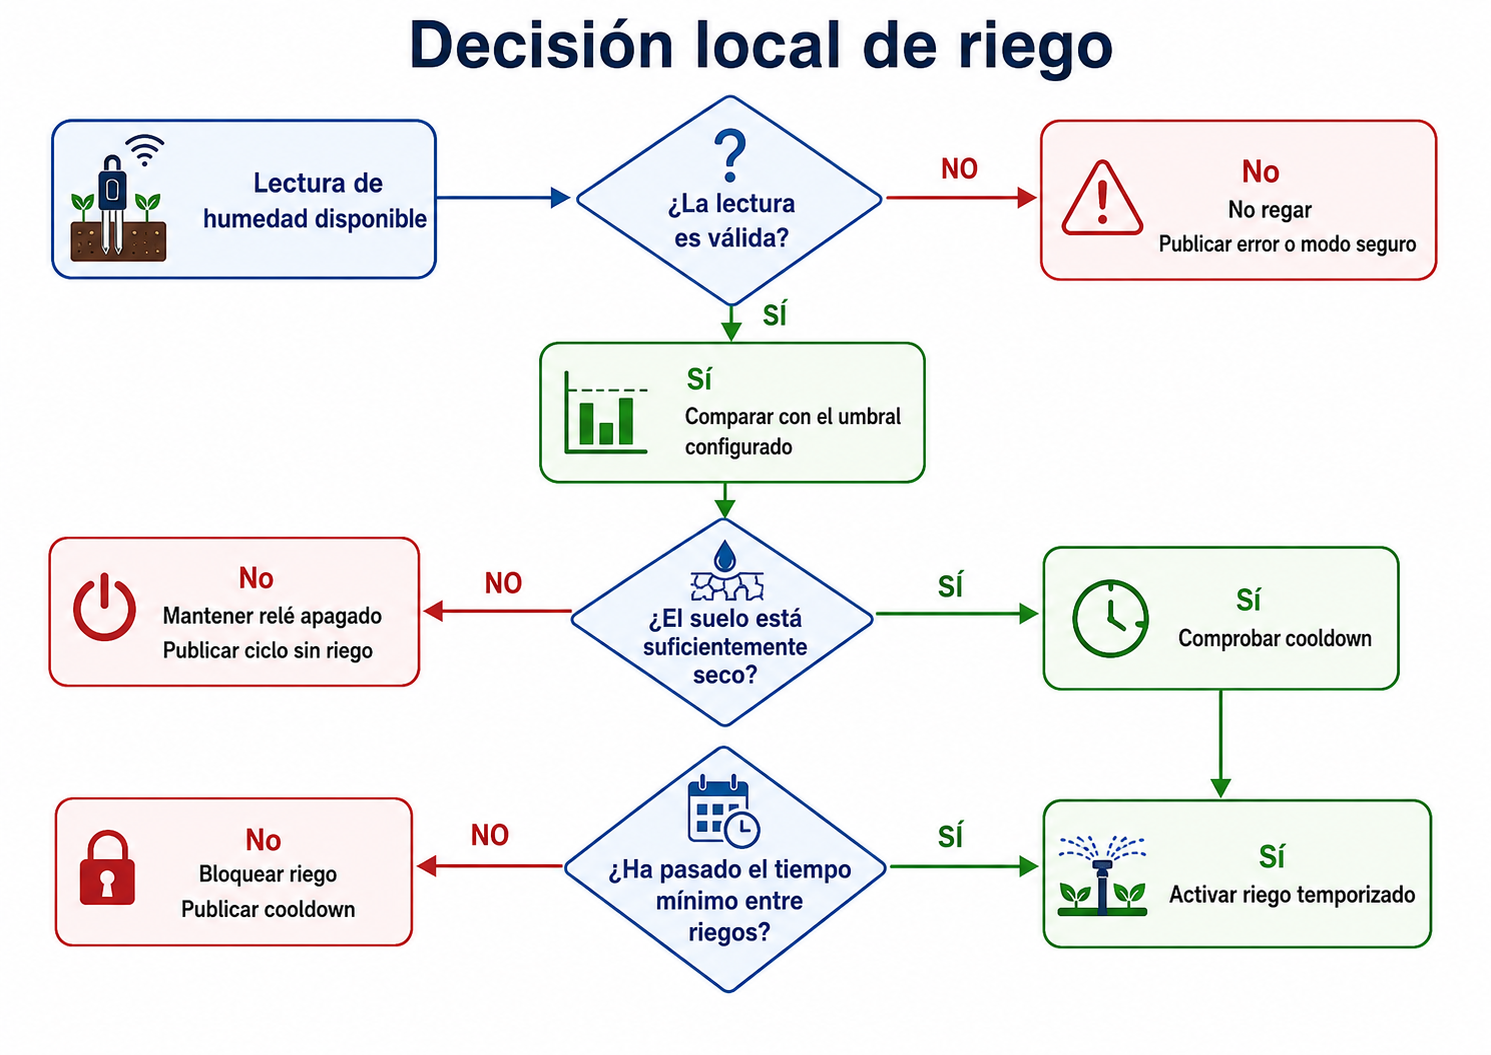
\includegraphics[width=0.75\textwidth]{figs_png/decision_local_riego_resumida.png}
        \caption{Flujo resumido de decisión local de riego.}
    \label{fig:decision_local_riego_resumida}
\end{figure}

La respuesta segura ante lectura inválida, error o \textit{cooldown} es mantener la bomba apagada.

\section{Supervisión en Raspberry Pi}

La Figura~\ref{fig:flujo_supervision_raspberry} resume el flujo seguido por la Raspberry Pi una vez que la estación ha publicado datos en ThingSpeak.

\begin{figure}[H]
    \centering
    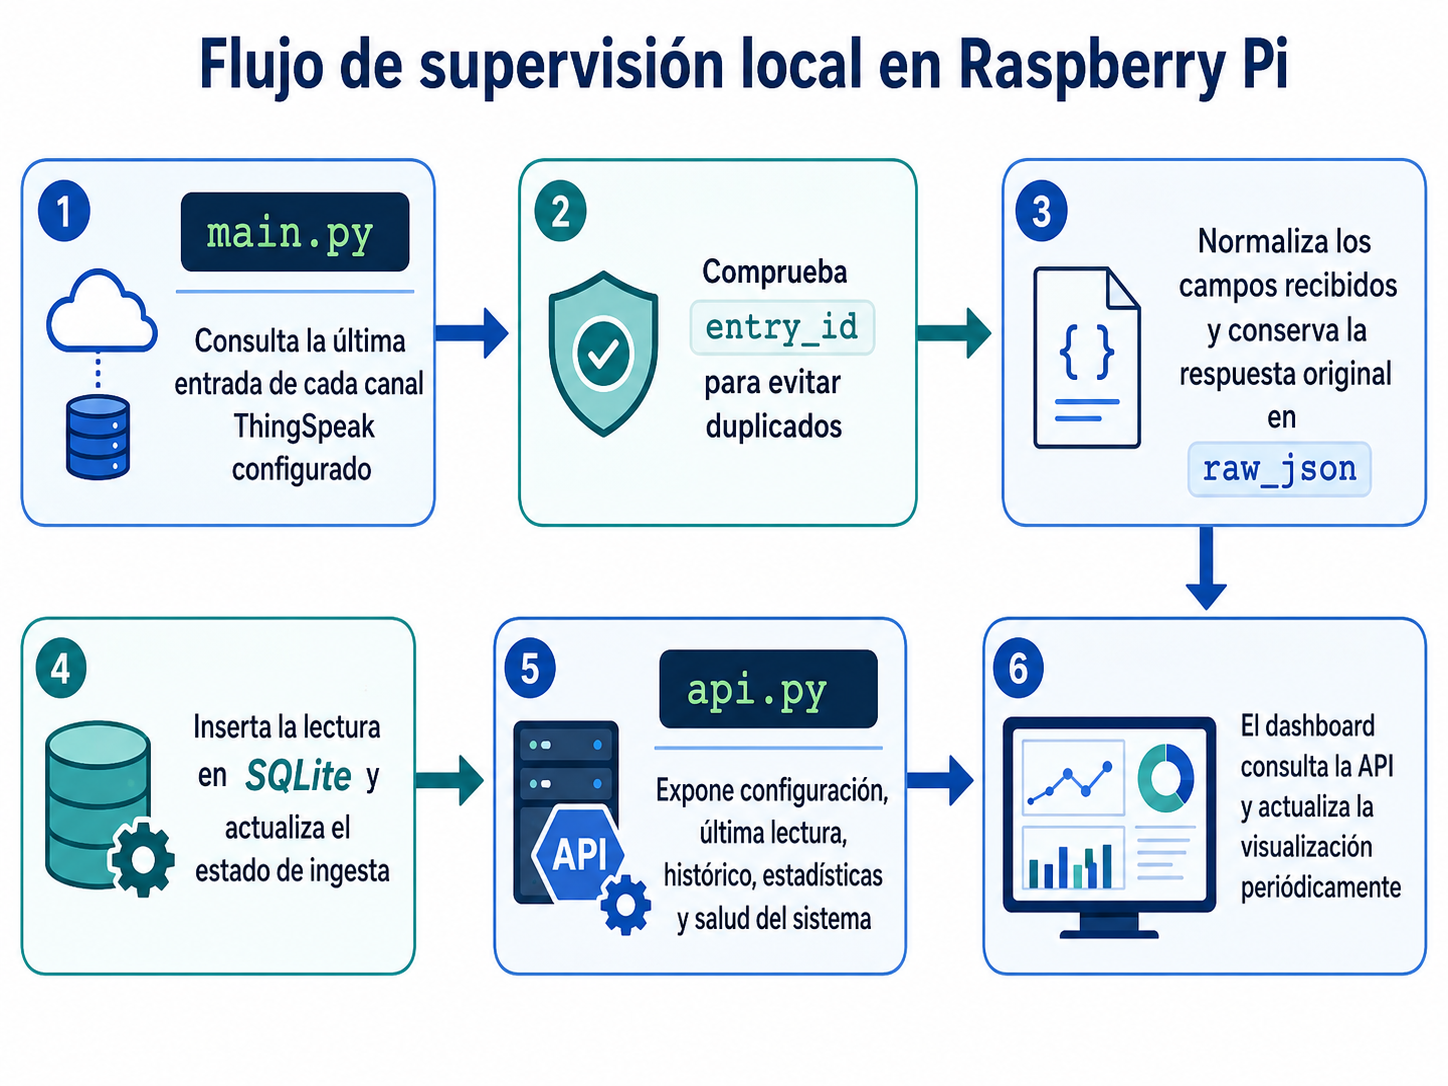
\includegraphics[width=0.7\textwidth]{figs_png/flujo_supervision_raspberry.png}
        \caption{Flujo de supervisión local en Raspberry Pi.}
    \label{fig:flujo_supervision_raspberry}
\end{figure}
    
Este flujo deja claro que la Raspberry Pi trabaja sobre datos publicados y almacenados. No se conecta físicamente a las estaciones ni acciona directamente el relé.

\section{Flujo ante fallos}

La Figura~\ref{fig:flujo_fallos_resumido} resume la respuesta esperada ante fallos relevantes.

\begin{figure}[H]
    \centering
    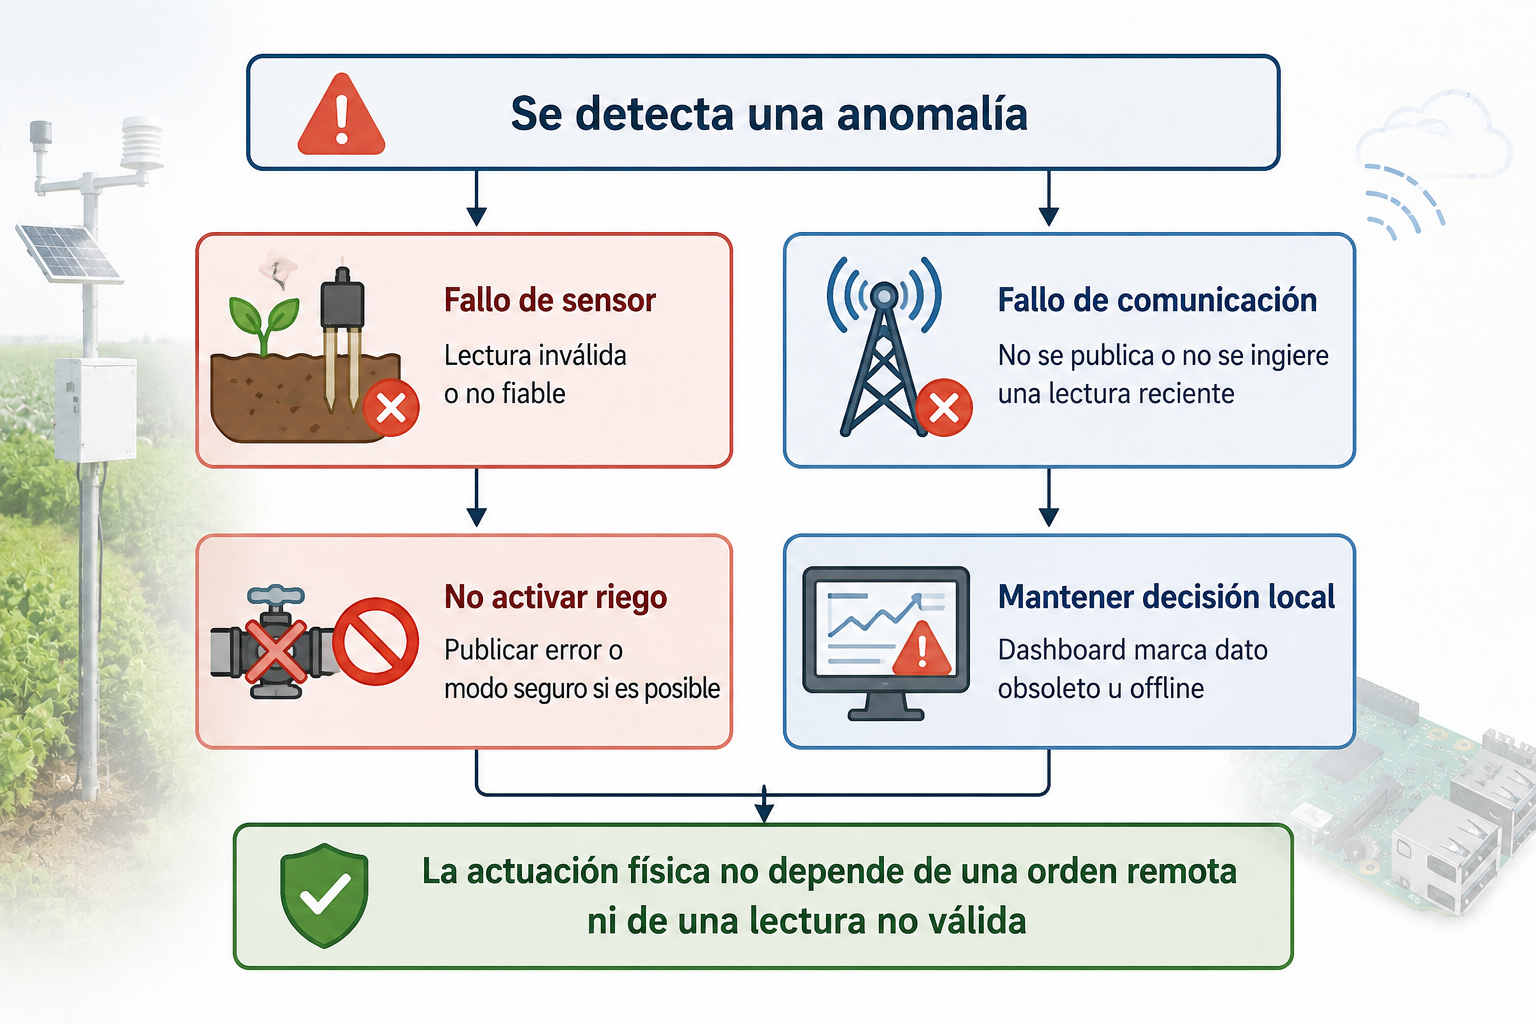
\includegraphics[width=0.7\textwidth]{figs_png/flujo_fallos_resumido.png}
        \caption{Flujo resumido ante fallos de sensor o comunicación.}
    \label{fig:flujo_fallos_resumido}
\end{figure}

La prioridad del sistema ante condiciones no fiables es mantener el estado seguro: relé apagado, riego no repetido y actuación limitada temporalmente.

\section{Secuencia extremo a extremo}

La Tabla~\ref{tab:secuencia_extremo_extremo_resumida} sintetiza la secuencia completa desde la medida física hasta la visualización.

\begin{table}[H]
\centering
\renewcommand{\arraystretch}{1.22}
\small
\begin{tabular}{|p{0.10\textwidth}|p{0.26\textwidth}|p{0.46\textwidth}|}
\hline
\rowcolor{gray!20}
\textbf{Paso} & \textbf{Elemento} & \textbf{Acción realizada} \\
\hline
1 & Sensores & Miden humedad del suelo, temperatura, humedad ambiental, luminosidad y presión. \\
\hline
2 & Arduino UNO & Valida lecturas y evalúa la lógica local de riego. \\
\hline
3 & Relé y bomba & Ejecutan el riego únicamente si se cumplen las condiciones y durante un tiempo limitado. \\
\hline
4 & A7670E-LASA & Publica telemetría y estado en ThingSpeak mediante LTE/HTTP. \\
\hline
5 & ThingSpeak & Almacena la entrada y asigna un \texttt{entry\_id}. \\
\hline
6 & Raspberry Pi & Recupera lecturas nuevas, evita duplicados y las guarda en SQLite. \\
\hline
7 & API & Expone los datos almacenados mediante \textit{endpoints} HTTP. \\
\hline
8 & \textit{Dashboard} & Muestra lecturas, estados, gráficas e histórico al usuario. \\
\hline
\end{tabular}
\caption{Secuencia extremo a extremo de TierraViva.}
\label{tab:secuencia_extremo_extremo_resumida}
\end{table}

\section{Responsabilidades por bloque}

La Tabla~\ref{tab:responsabilidades_bloques_resumida} resume las responsabilidades principales de cada capa del sistema.

\begin{table}[H]
\centering
\renewcommand{\arraystretch}{1.22}
\small
\begin{tabular}{|p{0.24\textwidth}|p{0.44\textwidth}|p{0.22\textwidth}|}
\hline
\rowcolor{gray!20}
\textbf{Bloque} & \textbf{Responsabilidad principal} & \textbf{Actúa físicamente} \\
\hline
Sensores & Medir variables del suelo y del entorno. & No \\
\hline
Arduino UNO & Leer sensores, validar datos, decidir riego y controlar el relé. & Sí \\
\hline
Relé y bomba & Ejecutar físicamente el riego cuando el \textit{firmware} lo permite. & Sí \\
\hline
A7670E-LASA & Enviar telemetría mediante LTE. & No \\
\hline
ThingSpeak & Recibir y conservar lecturas publicadas por las estaciones. & No \\
\hline
Raspberry Pi & Ingerir, almacenar y servir datos al \textit{dashboard}. & No \\
\hline
API FastAPI & Exponer lecturas, histórico, estadísticas y estado. & No \\
\hline
\textit{Dashboard} & Presentar información al usuario. & No \\
\hline
\end{tabular}
\caption{Responsabilidades principales de los bloques de TierraViva.}
\label{tab:responsabilidades_bloques_resumida}
\end{table}
